\section{Experiments}
\label{sec:exp}

\emph{Setup.} Offline numbers come from the frozen decision code (D-051, commit \tw{66917e7}), with older outputs re-run. Ranker evaluations use 761 val and 766 test lines from 26 and 27 held-out games. CIs are percentile intervals from 10,000 cluster-bootstrap resamples of whole games (seed 20261107), paired across models; exact McNemar $p$, which treats lines as independent, is the optimistic test. Thresholds, ensemble weights and feature-ranker configurations are chosen on val, so test is the clean column. % src: BM header; SA header

\subsection{Ranking the pro's play}
\label{sec:ranker}

\begin{table}[t]
\caption{4-way pick-the-pro-play accuracy (chance 0.25) with 95\% cluster-bootstrap CIs. ``Notes'' = tactics lines and per-option notes.}
\label{tab:ranker}
\centering\scriptsize
\setlength{\tabcolsep}{3pt}
\begin{tabular}{@{}lll@{}}
\toprule
Model & Val & Test\\
\midrule
\multicolumn{3}{@{}l}{\emph{Leak check and simple baselines}}\\
option-key rule, old options / 2$\times$2 grid & 0.853 / 0.250 & 0.852 / 0.250\\
random & 0.230 [0.207, 0.254] & 0.252 [0.218, 0.284]\\
popularity of the key & 0.468 [0.412, 0.516] & 0.325 [0.280, 0.374]\\
placement prior & 0.493 [0.430, 0.547] & 0.384 [0.337, 0.431]\\
\multicolumn{3}{@{}l}{\emph{Feature rankers, 783 features (seed 0)}}\\
logistic regression & 0.543 [0.492, 0.586] & 0.470 [0.423, 0.512]\\
LightGBM LambdaRank & 0.565 [0.520, 0.604] & 0.482 [0.448, 0.515]\\
\quad mean $\pm$ sd over 3 seeds & 0.5484 $\pm$ 0.0140 & 0.4913 $\pm$ 0.0126\\
DCN-V2 & 0.537 [0.493, 0.576] & 0.403 [0.366, 0.439]\\
\multicolumn{3}{@{}l}{\emph{d1-omni-600M decision LLM}}\\
zero-shot & 0.258 [0.226, 0.287] & 0.221 [0.191, 0.252]\\
ft-joint, plain lines & 0.524 [0.483, 0.561] & 0.483 [0.442, 0.522]\\
ft-joint, given notes it never saw & 0.477 [0.427, 0.523] & 0.461 [0.418, 0.506]\\
\textbf{ft-joint-tac} (trained on notes; live) & \textbf{0.547} [0.503, 0.584] & \textbf{0.507} [0.472, 0.540]\\
ft-joint-kg (also trained on \tw{KG:} lines) & 0.530 [0.480, 0.572] & 0.484 [0.450, 0.518]\\
\bottomrule
\end{tabular}
\end{table}
% src (Table ranker): SA sec. 1 (all CI rows); D-037 (0.853/0.852); feature_ranker_v2.md = feature_ranker_v1.md (3-seed mean); BM sec. 1 (option-set 0.250)

Table~\ref{tab:ranker} gives the main result. (1)~Zero-shot d1 is at chance: the 600M model has no usable Clash Royale knowledge, the parametric-memory limit of~\cite{mallen2023popqa,lim2026l11}. (2)~Fine-tuning lifts it 12.3 points above the placement prior on test ([+8.0, +16.7], $p<0.001$). (3)~The tuned feature ranker matches it: d1-ft-joint-tac minus LightGBM is +2.5 [$-$1.4, +5.9] (McNemar $p=0.263$), and $-$0.3 [$-$4.9, +4.0] against LightGBM's seed~2; LightGBM's top features by gain are the key's popularity (0.178) and $p(\text{zone}\mid\text{card})$ (0.124), the priors of the simple baselines. % src: SA sec. 2; feature_ranker_v2.md (gain 0.1782, 0.1240)
(4)~Training on the notes makes d1 robust to them, not reliant on them: notes hurt a model that never saw them, and on those lines the note-trained model beats it by +4.6 [+1.0, +8.4] ($p=0.006$), but its gain over the no-notes model on plain lines (+2.3 [$-$0.9, +5.3]) is not significant, and deleting its notes does not lower its accuracy (Sec.~\ref{sec:conflict}). % src: SA sec. 2 (+4.6, +2.3); CC replicate (C1)
(5)~Retraining with \tw{KG:} lines did not help ($-$2.2 [$-$4.7, +0.5]): validation loss rose from 1.1916 to 1.6708 in epoch 2, and the KG facts on training lines are mined from the same games, a leak we have not removed. % src: SA sec. 2; CMA C4 (val loss); CMA A2 RETRO row (FIX_LIST #49)

\begin{figure}[t]
\centering
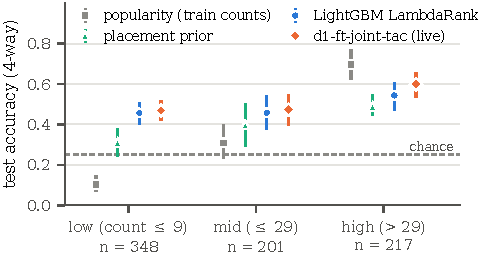
\includegraphics[width=\columnwidth]{figs/fig_popularity.pdf}
\caption{Test accuracy by training frequency of the gold key (terciles; 95\% cluster-bootstrap CIs). Popularity wins on head keys and fails on the tail; the fine-tuned LLM and LightGBM hold up on rare keys. Data: \tw{stats\_audit\_v1.json}.}
\label{fig:popularity}
\end{figure}

By training frequency of the gold key (Fig.~\ref{fig:popularity}), popularity is the best model on head keys (0.696) and the worst on the tail (0.103), while d1-ft-joint-tac and LightGBM stay level across the two lower terciles (0.468/0.473, 0.457/0.458), generalising beyond memorised keys; a share of 0.14 of test gold keys never occurs in training. % src: SA sec. 5

d1 is well calibrated (test ECE 0.048 over 15 bins; Brier 0.616): holding when its top probability is below 0.483 (chosen on val) answers 0.402 of test lines at 0.630 accuracy and raises the +1/0/$-$1 CRAG-style utility~\cite{yang2024cragbench} from 0.013 [$-$0.056, 0.079] to 0.104 [0.060, 0.147] (Fig.~\ref{fig:retsel}b). A d1+LightGBM ensemble changes test accuracy by $-$0.1, +2.1 or +3.9 points depending on LightGBM's seed, so we do not claim it; a rule arbiter narrowing d1's options when it is unsure gives no gain (0.509 vs 0.506) and stays off. % src: SA sec. 3, 4, 6; arbiter_v2.md (50.6% / 50.9%)

\subsection{Decision models}
\label{sec:decmodels}

\begin{table}[t]
\caption{Decision models on the 766 test lines of Table~\ref{tab:ranker} (game-bootstrap CIs, seed 0; d1's 0.5065 shows there as 0.507); middle block zero-shot. All differ from d1-ft-joint-tac at McNemar $p<0.001$ but LightGBM ($p=0.263$). $^\dagger$Thinking \tw{between\_tools}, $\le$2,000 output tokens, answer parsed from the end; with the 16-token cap of the other API runs 62.8\% of Sonnet replies were cut off (accuracy 0.144), 3.8\% of Haiku's (counted wrong).}
\label{tab:decmodels}
\centering\scriptsize
\setlength{\tabcolsep}{2.2pt}
\begin{tabular}{@{}llccc@{}}
\toprule
Model & Accuracy [95\% CI] & Card & ms p50/p95 & US\$/dec.\\
\midrule
\textbf{d1-ft-joint-tac}, 600M (live) & \textbf{0.506} [0.473, 0.538] & 0.692 & 75/117 & 0\\
d1-2B fine-tuned, 1.9B & 0.429 [0.394, 0.466] & 0.614 & 295/465 & 0\\
\midrule
d1-omni-600M zero-shot & 0.260 [0.235, 0.283] & 0.513 & 73/113 & 0\\
Qwen3-4B-Instruct-2507 & 0.286 [0.244, 0.331] & 0.527 & 802/1119 & 0\\
\quad + 3 retrieved pro states & 0.283 [0.251, 0.316] & 0.516 & 1535/1958 & 0\\
Qwen3-14B & 0.304 [0.264, 0.345] & 0.523 & 2721/3866 & 0\\
Claude Haiku 5.5 & 0.279 [0.250, 0.310] & 0.499 & 676/823 & 0.00009\\
Claude Sonnet 5.5$^\dagger$ & 0.364 [0.325, 0.403] & 0.585 & 2467/4824 & 0.00369\\
\midrule
LightGBM LambdaRank & 0.482 [0.448, 0.514] & 0.677 & 0.4/0.5 & 0\\
placement prior & 0.384 [0.336, 0.431] & 0.614 & 0.003/0.003 & 0\\
popularity & 0.325 [0.280, 0.373] & 0.453 & 0.001/0.002 & 0\\
random, one draw (exp.\ 0.250) & 0.269 [0.237, 0.301] & 0.539 & 0.001/0.001 & 0\\
\bottomrule
\end{tabular}
\end{table}
% src (Table decmodels): docs/data/decision_models_v1.md "Accuracy and latency" (every cell; Sonnet row = claude-sonnet-5-5-long,
%   the claude-sonnet-5-5 row gives 0.144 and 481/766 = 62.8% parse failures; Haiku 29/766 = 3.8%; random (expected) 0.250 / 0.500);
%   decision_models_v1.json models.d1-ft-joint-tac.acc.est = 0.5065, models.lightgbm.vs_reference.mcnemar_p = 0.26333;
%   Sonnet settings and "max_tokens" errors: tools/eval/bench_claude_rankers.py VARIANTS, runs/bench/au/preds/claude-*.jsonl

\emph{Protocol} (MAC-AU). The LLMs share one prompt: d1's input (state text with \tw{tactics:} and \tw{KG:} lines, options A--D with notes) and a request for the pro's choice. Qwen3~\cite{qwen2025qwen3} decodes greedily, Claude Haiku with 16 output tokens, both thinking off (Sonnet: $^\dagger$); the RAG variant prepends the 3 nearest train-split pro states (600 characters each, plus the pro's play). Latency is wall time per decision after a warm-up (M5: d1 on MPS, Qwen in MLX 4-bit, one model at a time; API: with the network); cost is usage times list price. % src: docs/plans/MAC-AU_decision_models_retrieval_benchmark.md (Part A prompt, Qwen, RAG, Claude, GPU discipline, Amendment 1); tools/eval/bench_llm_rankers.py (greedy, 8 new tokens, enable_thinking False); decision_models_v1.md header (latency definition)

\emph{Findings.} Fine-tuning dominates. Zero-shot, d1-omni-600M, both Qwen3 models and Claude Haiku 5.5 stay within 5.4 points of chance, the parametric-memory limit~\cite{mallen2023popqa,lim2026l11} (d1: 0.260 with notes, 0.221 without, Table~\ref{tab:ranker}). Claude Sonnet 5.5, the best zero-shot model, is 14.2 points [$-$19.1, $-$9.3] below the fine-tuned 600M at 33$\times$ its median latency and a per-decision cost: RankGPT-style zero-shot ranking~\cite{sun2023rankgpt,cap6938L10} falls short in this domain and budget. Three retrieved pro examples (RAG few-shot~\cite{lim2026l11}) do not help Qwen3-4B (0.283 vs 0.286) and nearly double its latency. The larger fine-tune is worse: d1-2B (top 8 layers trained, val 0.4192) loses 7.7 points [$-$12.2, $-$3.4] at 4$\times$ latency. LightGBM, a tuned baseline~\cite{rendle2020ncfvsmf,lim2026l13}, is on par at 0.4\,ms. % src: decision_models_v1.md (accuracies; diff column: Sonnet-long -0.142 [-0.191, -0.093], d1-2B -0.077 [-0.122, -0.034], LightGBM -0.025 [-0.059, +0.014]; latency p50 2467 / 75 = 33x, 295 / 75 = 3.9x, 1535 / 802 = 1.9x); 0.304 - 0.25 = 5.4 pts (Qwen3-14B, largest of the four); CMA C4 (d1-2B top 8 layers, val 0.4192); SA sec. 1 (0.221); CMA A2 parametric-memory row (d1_zero_shot_v1.json joint = plain lines, 0.2206 test)

\subsection{Retrieval}
\label{sec:retr}

\begin{table}[t]
\caption{Retrieval channels (916/902 val/test queries, train pool, depth 50). Hit@10: the pro's exact play is among the top-10 neighbours' plays.}
\label{tab:retrieval}
\centering\scriptsize
\setlength{\tabcolsep}{3pt}
\begin{tabular}{@{}lccc@{}}
\toprule
List & hit@10 val / test & card hit@10 val / test & ms p50 (test)\\
\midrule
BM25 (FTS5) & 0.142 / 0.159 & 0.396 / 0.483 & 25.8\\
structured kNN (644-d) & 0.166 / 0.136 & 0.434 / 0.412 & 2.1\\
text (bge-small, 384-d) & 0.132 / 0.143 & 0.397 / 0.436 & 22.2\\
struct + BM25 (live) & 0.138 / 0.160 & 0.434 / 0.487 & 28.0\\
all three, RRF & 0.156 / 0.170 & 0.461 / 0.514 & 49.6\\
\bottomrule
\end{tabular}
\end{table}
% src (Table retrieval): docs/data/retrieval_ablation_v1.md (kept current per BM sec. 3)

Table~\ref{tab:retrieval}: the channels are within noise (test hit@10 0.136--0.170); BM25 beats the structured channel on test (0.159 vs 0.136) but not on val, and the text channel adds about 20\,ms for no clear gain, so the live list is structured plus BM25. As a lone candidate source, kNN voting loses to popularity on exact keys (test recall@10 0.317 vs 0.402) and wins only on cards (0.651 vs 0.607). % src: CMA A1 (ranker_baselines_v1.json candidate_recall)
HNSW at ef 40 keeps recall@10 at 0.978 in 0.31 vs 1.51\,ms for exact search (Fig.~\ref{fig:retsel}a), but at 10.9k vectors exact search stays live. For pre- vs post-filtering~\cite{cap6938L09}, a deck pre-filter empties the pool for 88.9\% of queries (decks unseen in training); post-filtering the top 10 returns nothing for 50.0\% (deck) and 87.3\% (phase) of queries, the top 200 for 0.5\% and 0.1\%. % src: retrieval_ablation_v1.md (HNSW table, filtering table)

\begin{figure}[t]
\centering
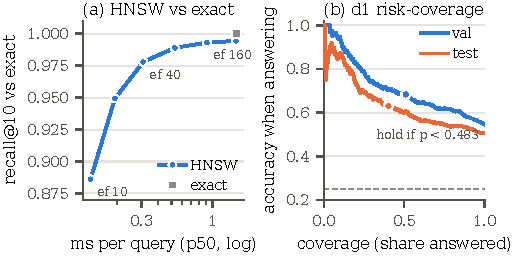
\includegraphics[width=\columnwidth]{figs/fig_retrieval_selective.pdf}
\caption{(a) HNSW recall@10 against exact kNN versus query time (10,923 vectors, $k{=}10$). (b) Risk--coverage of d1-ft-joint-tac holding below a probability threshold (dots: 0.483, set on val).}
\label{fig:retsel}
\end{figure}

\subsection{KG embeddings and mined rules}
\label{sec:kg}

\begin{table}[t]
\caption{Held-out COUNTERS link prediction, test (762 queries, filtered, 3 seeds).}
\label{tab:kg}
\centering\scriptsize
\setlength{\tabcolsep}{3pt}
\begin{tabular}{@{}lccc@{}}
\toprule
Method & MRR & H@1 & H@10\\
\midrule
random & 0.0223 & 0.0113 & 0.1129\\
popularity & 0.1103 & 0.0381 & 0.2385\\
TransE & 0.0819 $\pm$ 0.0046 & 0.0000 & 0.2380\\
DistMult & 0.0907 $\pm$ 0.0083 & 0.0232 & 0.1986\\
ComplEx & 0.1162 $\pm$ 0.0074 & 0.0367 & 0.2616\\
RotatE & \textbf{0.1588} $\pm$ 0.0020 & 0.0713 & 0.3259\\
\bottomrule
\end{tabular}
\end{table}
% src (Table kg): docs/data/kge_link_prediction_v1.md (setting full). The former part (b), E6 test hit@1 / MRR, is identical to Table retrmethods (b)
%   rows v2 full / pro only / v1 wiki COUNTERS / popularity / random (answer_rules_v1.md test table = retrieval_methods_v1.md KG table)

\emph{Link prediction} (Table~\ref{tab:kg}). We hold out wiki COUNTERS triples (3,043/380/381) and rank 126 candidate cards (filtered, tie-aware); all four PyKEEN~\cite{ali2021pykeen} models get the same grid (dimension 32 or 64, learning rate 0.01 or 0.001; chosen on val MRR) and three seeds, per the course's evaluation-audit protocol~\cite{ruffinelli2020olddog,sun2020reevaluation,cap6938L05}. RotatE~\cite{sun2019rotate} is best and beats popularity; TransE and DistMult do not, DistMult being symmetric by construction (asymmetry score 0.0) while only 940 of 3,804 counter pairs have a reverse edge. % src: CMA A3 (triples, grid, asymmetry, 940 / 3,804); kge_link_prediction_v1.md

\emph{Mined answer rules} (E6; test in Table~\ref{tab:retrmethods}b). For each of 609/433 held-out val/test events we rank the pro's own deck (7.96/7.83 cards on average) with rules mined from training games (support $\ge3$, 8\,s window); val hit@1: full 0.182, pro-mined only 0.191, wiki COUNTERS 0.117, train popularity 0.182, random 0.126. Pooled over val and test, the full score beats random (+0.044 hit@1 [+0.020, +0.068]) and the wiki counters (+0.043 [+0.011, +0.074]) but not the training popularity of the answer card ($-$0.006 [$-$0.035, +0.020]); on test the pro-mined source alone falls below popularity ($-$0.040 hit@1, $p=0.022$). The score barely predicts whether the answer held the tower (AUROC 0.543), few rules have large support (10 or more for 63 of 1,042 events), and 8\,s is the best window of 2, 4 and 8\,s on val (MRR 0.409). Unlike AMIE and TLogic, which score rules on their mining data~\cite{lajus2020amie3,liu2022tlogic}, this held-out test against popularity~\cite{ruffinelli2020olddog} shows the 287 rules mostly re-encode the pro's card frequencies, a weak prior~\cite{cap6938L07}. % src: answer_rules_v1.md (headline val table: 0.182, 0.191, 0.117, 0.182, 0.126; 609 / 433 events; paired val+test, test paired, AUROC, strata, sweep)

\subsection{Retrieval methods for the KB and the KG}
\label{sec:retrmethods}

\begin{table}[t]
\caption{KB and KG methods on the 766 test lines, retrieving from train games. (a)~KB, top 20: a hit's pro play has the gold key (hit@10, MRR) or card (card@10); rec.\ = overlap with exact top 20. (b)~KG: 433 held-out threat$\rightarrow$answer events, ranked over the pro's deck. 4-way: accuracy as a decision model (unsupported lines tied); Cov.: share of lines supported; ms: query p50. Two options share each card: a card-level score is capped at 0.5 4-way.}
\label{tab:retrmethods}
\centering\scriptsize
\setlength{\tabcolsep}{2.4pt}
\begin{tabular}{@{}lcccccc@{}}
\toprule
(a) KB method & hit@10 & card@10 & MRR & 4-way & Cov. & ms\\
\midrule
dense exact (644-d, dot) & 0.144 & 0.423 & 0.067 & 0.284 & 0.53 & 1.16\\
BM25 (FTS5) & 0.166 & 0.491 & 0.060 & \textbf{0.318} & 0.53 & 22.14\\
RRF dense + BM25 (live) & 0.175 & 0.501 & 0.074 & 0.305 & 0.58 & 24.19\\
bge-small text (cosine) & 0.155 & 0.450 & 0.067 & 0.307 & 0.46 & 13.64\\
RRF all three & \textbf{0.184} & \textbf{0.530} & \textbf{0.082} & 0.314 & 0.54 & 45.16\\
HNSW ef 10 (rec.\ 0.977) & 0.141 & 0.418 & 0.067 & 0.287 & 0.52 & 0.84\\
HNSW ef 40 (rec.\ 0.990) & 0.141 & 0.419 & 0.067 & 0.286 & 0.53 & 1.11\\
HNSW ef 160 (rec.\ 0.998) & 0.142 & 0.422 & 0.067 & 0.286 & 0.53 & 2.24\\
deck pre-filter, then dense & 0.076 & 0.157 & 0.041 & 0.286 & 0.16 & 0.82\\
\midrule
(b) KG method & hit@1 & hit@3 & MRR & 4-way & Cov. & ms\\
\midrule
v1 \tw{counter\_scores} & 0.143 & 0.409 & 0.360 & 0.249 & 0.31 & 0.01\\
v1 wiki COUNTERS only & 0.141 & 0.406 & 0.359 & 0.250 & 0.29 & 0.01\\
v2 \tw{answers\_for}, full & 0.154 & 0.422 & 0.374 & 0.239 & 0.45 & 0.05\\
\quad pro source only & 0.129 & 0.399 & 0.350 & 0.236 & 0.20 & 0.04\\
\quad role transfer only & 0.145 & 0.398 & 0.356 & 0.241 & 0.24 & 0.04\\
\quad wiki only & 0.147 & 0.407 & 0.362 & 0.249 & 0.29 & 0.04\\
\quad simulation (STOPS) only & 0.157 & \textbf{0.440} & 0.376 & \textbf{0.258} & 0.31 & 0.04\\
KGE RotatE & 0.125 & 0.400 & 0.340 & 0.253 & 0.49 & 0.18\\
KGE TransE & 0.118 & 0.353 & 0.335 & 0.245 & 0.49 & 0.13\\
train popularity of the answer & \textbf{0.169} & 0.433 & \textbf{0.384} & 0.217 & 0.49 & 0.00\\
random (expected) & 0.128 & 0.384 & 0.345 & 0.250 & -- & --\\
\bottomrule
\end{tabular}
\end{table}
% src (Table retrmethods): docs/data/retrieval_methods_v1.md, "KB: the pro-state database" (hit@10, card_hit@10, MRR, 4-way acc,
%   coverage, recall@20 vs exact, ms p50) and "KG: threat to answer" (hit@1, hit@3, MRR, 4-way acc, line coverage, query ms p50);
%   433 events / 374 lines with a threat, train-only pool and leak check, card-level cap 0.5: same file, "Setup and leakage"

As retrievers (Table~\ref{tab:retrmethods}a) the hybrids lead (\cf Sec.~\ref{sec:retr} and~\cite{cap6938L08,cap6938L09,cap6938L10}): RRF of all three lists has the best hit@10, card@10 and MRR, and the live dense+BM25 fusion beats both its lists (hit@10 0.175 vs 0.144, 0.166), with overlapping CIs. HNSW keeps 0.977--0.998 of the exact top 20, but over 4,997 train states exact search takes only 1.16\,ms (ef 10 saves 0.3\,ms). The deck pre-filter returns nothing for 78.3\% of lines (decks unseen in train; the pre-filter risk of~\cite{cap6938L09}), though on the 16\% it supports it is the most accurate KB rule (0.475). % src: retrieval_methods_v1.md KB table (recall@20, ms, empty 0.783, acc if supported 0.475 [0.312, 0.587]) and Setup (4,997 train states with an action); 1.16 - 0.84 = 0.32 ms
No method alone is a usable decision maker: the best, BM25, reaches 0.318 [0.283, 0.351], 18.9 points below d1, other KB methods 19--22 and the KG methods 25--29 points below (all McNemar $p<10^{-12}$), as a card-level score cannot place and finds a threat on 374 of 766 lines; no KG method beats train popularity on hit@1 or MRR (0.169, 0.384). Their value is as candidate sources and ranker context (Sec.~\ref{sec:disc}). % src: retrieval_methods_v1.md "Retrieval as a decision model" (delta vs d1: KB -0.189 to -0.222, KG -0.248 to -0.289; largest McNemar p 2.28e-13), Headline (BM25 0.318 [0.283, 0.351]; popularity MRR 0.384)

\subsection{Context conflict: does d1 follow notes? (E2)}
\label{sec:conflict}

Following ClashEval and the knowledge-conflict lecture~\cite{wu2024clasheval,xie2024chameleon,lim2026l17}, we corrupt d1-ft-joint-tac's context with the gold label fixed: C1 removes the notes and \tw{tactics:}/\tw{KG:} lines; C2 shuffles the notes across options; C3 swaps the gold option's informative note with a distractor's and names a wrong card in the \tw{tactics:} line (relevant but misleading); C4 transplants another line's tactics/KG block (irrelevant). Follow-rate: the share of movable lines (the corruption favours an option d1 did not pick) whose pick moves to the favoured option.

\begin{table}[t]
\caption{Context conflict on d1-ft-joint-tac (E2), test lines (n = 766, 27 games), 95\% cluster-bootstrap CI; $p$ = exact McNemar; follow-rate as in the text (C4: 12 movable lines).}
\label{tab:conflict}
\centering\scriptsize
\setlength{\tabcolsep}{3pt}
\begin{tabular}{@{}lllcc@{}}
\toprule
Condition & Accuracy [CI] & $\Delta$ pts ($p$) & Changed & Follow\\
\midrule
C0 as exported & 0.507 [0.473, 0.539] & -- & -- & --\\
C1 context removed & 0.508 [0.476, 0.541] & +0.1 (1.00) & 21\% & --\\
C2 notes shuffled & 0.517 [0.482, 0.550] & +1.0 (0.27) & 7\% & 0.094\\
C3 notes poisoned & 0.503 [0.469, 0.535] & $-$0.4 (0.76) & 6\% & 0.044\\
C4 block transplanted & 0.495 [0.459, 0.530] & $-$1.2 (0.45) & 19\% & 0.083\\
\bottomrule
\end{tabular}
\end{table}
% src (Table conflict): docs/data/context_conflict_v1.md, replicate on joint_tac_v2 (HEAD notes, same lines as Table III), "Accuracy by condition - test" and "Follow-rate - test"; p = exact McNemar

Table~\ref{tab:conflict}: no condition moves accuracy by more than 1.2 points. Removing the whole context changes 21\% of picks, but gains and losses cancel (57 vs 56 lines); poisoned notes move 4.4\% [2.1, 6.8] of movable picks. Lines whose gold option carries the informative note are easier than lines where a distractor's does (0.564 vs 0.371), but the gap persists with no notes (0.599 vs 0.401), so it reflects which states are easy. Context-aware decoding~\cite{shi2024cad} selects weight $a=0$ on val in every condition, and each $a>0$ lowers C0 test accuracy by 1.7 to 2.9 points; AdaCAD's adaptive weight~\cite{wang2025adacad} averages 0.014 and changes accuracy by $-$0.1 points. % src: CC replicate joint_tac_v2 (test tables, strata, CAD C0)
d1 thus avoids both failures the course warns about, adopting wrong context over its prior (ClashEval~\cite{wu2024clasheval}) and greater sensitivity to relevant-but-misleading than to irrelevant noise (RAGChecker~\cite{ru2024ragchecker}), because it barely reads its notes, plausibly as they favour the gold option on only 30\% of test lines and a distractor on 22\% (49\% have none), so it is robust to wrong tool output. % src: CC replicate test note status (227 right, 167 wrong, 372 none of 766)

\subsection{When to act}
\label{sec:timing}

On dense test seconds (n = 5,279), balanced accuracy for ``the pro deploys within $h$'' at $h$ = 1/2/3\,s is 0.506/0.509/0.510 for the hand-written rules and 0.594/\textbf{0.607}/0.613 for LightGBM on 29 features (AUC 0.632/0.659/0.672); the live \emph{fast} combination, with rules overriding the model in four modes, sits between them (0.571/0.584/0.593). % src (Table timing): docs/data/act_gbdt_v2.md overview + apples-to-apples test table; act_head_v2.md (0.558, unchanged from v1)
On the balanced subset ($h=1$\,s, n = 3,221) used to train a d1 act head (top 8 layers, 168.9M trainable parameters), LightGBM scores 0.598 against the head's 0.558, at 0.05\,ms instead of about 70\,ms per call: again the tuned simple model beats the LLM. % src: act_gbdt_v2.md (apples-to-apples test table); act_head_v2.md (0.558); CMA B (act head 168.9M, ~70 ms), C4

\subsection{Next card, opponent deck, knowledge editing}

For opponent next-card prediction, a sequential recommendation task~\cite{kang2018sasrec,lim2026l14}, SASRec (3 seeds) reaches acc@1 0.129/0.222 on val/test and loses to a copy-frequency rule (0.207/0.243), the copy intuition of CyGNet~\cite{zhu2021cygnet,cap6938L06C}; popularity is near zero (0.000/0.002) because opponents vary, and the ceiling set by cards already seen is 0.678/0.644. The KG opponent-deck model recovers hidden cards with recall 0.234/0.291/0.327 after 1/2/3 seen cards, against 0.130/0.124/0.118 for popularity (leave-one-game-out, 155 games). % src: next_card_v1.md; opp_model_v1.md (BM sec. 7)
For knowledge editing~\cite{yao2023editingsurvey,lim2026l17} we apply a synthetic +1-elixir patch to five cards in a patch-versioned fact store, SERAC's non-parametric route~\cite{mitchell2022serac}: reliability, generalisation and portability are 1.000 (0.000, 0.000, 0.067 without the edit), locality 1.000, rollback passes, and re-weighting cuts retrieved hits using an edited card from 0.124 to 0.002; the store is deterministic, so this shows the mechanism, not that it generalises to a real patch~\cite{yang2025mirage}. % src: edit_eval_v2.md (identical to edit_eval_v1.md)

\subsection{Bot versus pro on held-out videos}

We run the live stack open loop on held-out test videos with the pro's deck and a dry-run executor, matching its would-be taps to the pro's plays within $\pm$2\,s. As taps do not change the video, this measures what the bot would do in the pro's place, not whether it would win (its hand memory never learns a card left the hand). Retrieval uses only train and val games, the KG answers and placement prior only train games. Results cover the 24 usable test games (90\,min, 1,561 pro plays, 2,042 bot taps); 4 more lack a full deck. % src: VP header and "Not run" list

\begin{table}[t]
\caption{Bot vs pro on held-out pro videos, open loop: 24 test games, 1,561 pro plays. Percent; window $\pm$2\,s; 95\% CIs by game bootstrap. Null: the bot's own taps shifted by 20--60\,s. Baselines use the same plays; the placement prior is given the pro's card.}
\label{tab:vspro}
\centering\scriptsize
\setlength{\tabcolsep}{3pt}
\begin{tabular}{@{}lll@{}}
\toprule
Measure & Bot [95\% CI] & Baseline\\
\midrule
pro plays met by a bot tap & 77.1 [71.8, 83.0] & 68.9 (null)\\
bot taps met by a pro play & 72.6 [69.3, 76.2] & 67.9 (null)\\
taps (bot) / plays (pro) per min & 22.8 [20.2, 25.9] & 17.4 [16.5, 18.4]\\
same card, matched pairs & 17.1 [14.6, 20.2] & 12.8 (random in hand)\\
same card, KG threat exists (126) & 19.8 [13.3, 26.9] & 15.6 (KG v1 counter)\\
pro's card in perceived hand & 40.1 [37.3, 43.2] & 53.0 (dataset's hand)\\
same lane $\mid$ same card (103) & 42.7 [31.6, 53.5] & 44.6 (placement prior)\\
same key $\mid$ same card (103) & 26.2 [16.8, 36.0] & 29.7 (placement prior)\\
\bottomrule
\end{tabular}
\end{table}
% src (Table vspro): docs/data/vs_pro_v1.md (MAC-AQ, generated 2026-11-08T02:31:35Z, all 24 usable test games) Headline table (every cell, subset sizes 126 and 103) and Timing table.

Table~\ref{tab:vspro}: the bot's timing beats the null (matched taps a median 0.47\,s from the pro's play), which matters because it taps more often and spends more elixir than the pro (58.7 vs 33.6 per minute). Its card choice beats a random card of its hand and, where a KG threat exists, the KG v1 counter rule, but the ceiling is low: the pro's card is in the perceived hand on only 40.1\% of plays, and the bot cannot pick a card it does not see. Missed pro plays were mostly held because no card was affordable (23.0\%), the engine left the push to the tower (22.7\%) or the act model waited (18.8\%). % src: VP Headline, Timing (0.47 s; elixir/min 58.72, 33.58), When the bot held

\subsection{Live play and prior bots}
\label{sec:live}

\begin{table}[t]
\caption{(a) Latency by stage, ms p50 / p95: live trial session (363 decisions) and mean of 3 video dry runs ($\pm$ sd for the total; a shared Mac, so upper bounds). (b) Live record in Training Camp.}
\label{tab:live}
\centering\scriptsize
\setlength{\tabcolsep}{3pt}
\begin{tabular}{@{}lcc@{}}
\toprule
(a) Stage & trial session & dry run, 3 reps\\
\midrule
capture & 22.0 / 44.8 & 0.8 / 4.3\\
perception (detector, OCR, hand) & 108.0 / 266.4 & 179.2 / 234.2\\
live state & 0.13 / 0.31 & 0.2 / 0.5\\
trigger (rules + LightGBM) & 1.1 / 9.2 & 2.7 / 9.7\\
candidates (engine, retrieval, KG) & 26.8 / 57.9 & 46.7 / 86.1\\
rank (d1; 0 when one candidate) & 0.0 / 140.9 & 87.1 / 191.0\\
execute (two clicks) & 181.0 / 188.8 & no clicks\\
\textbf{total} & \textbf{322.7 / 601.6} & 271.7$\pm$20.1 / 455.2$\pm$41.2\\
\midrule
\multicolumn{3}{@{}l}{(b) Live record}\\
\midrule
runs before the trial, 11-03 to 11-07 & \multicolumn{2}{l}{13 (12 live), 931 decisions, 746 taps}\\
taps landed, two newest of them & \multicolumn{2}{l}{75/84, 78/95 (older run 233907: 95/100)}\\
run 013441 (3 battles) & \multicolumn{2}{l}{tower taken; 3-crown loss; \textbf{win in overtime}}\\
\textbf{trial}: wins / battles, exact CI & \multicolumn{2}{l}{\textbf{0 / 10}, 95\% CI 0--30.8\%}\\
\quad crowns for / against (10 battles) & \multicolumn{2}{l}{3 / 18; a tower taken in 3; 2 in overtime}\\
\quad per logged battle (9 of 10) & \multicolumn{2}{l}{40.3 decisions, 27.0 taps; median 213\,s}\\
\bottomrule
\end{tabular}
\end{table}
% src (Table live): (a) trial-session column: LOG decisions.jsonl timings_ms, all 363 rows, nearest-rank p50 / p95 (total 322.7 / 601.6);
%   dry-run column: LAT "Whole stack, 3 repeated dry runs" (video Z8-4VhLjrGU 60-180 s, runs/rerun/lat_{1,2,3}), mean of p50 / p95, sd for total
%   (b) CMA C6 = BM sec. 13 (12 live runs, 931, 746) + LAT (dry run 20261105-205720); BM sec. 11 (tap_landing_20261107-013441_v2.md 75/84,
%   tap_landing_20261107-111554_v2.md 78/95, tap_landing_233907_v1.md 95/100); STATUS 2026-11-07 night (run 013441);
%   trial rows: TRIAL (0/10, scores, crowns 3/18, 2 OT, 3 with a tower; Clopper-Pearson 0-30.8%, checked with scipy beta.ppf(0.975,1,10) = 0.3085);
%   LOG battles.jsonl (9 TRAINING_CAMP rows: 363 decisions, 243 taps, median duration 212.6 s) and decisions.jsonl timings_ms (total 323/602)

The 13 runs before the trial (Table~\ref{tab:live}b; 12 live, one dry) took 347/613\,ms p50/p95 in total (339/572\,ms in run 111554). In the trial (Table~\ref{tab:live}a) perception (108\,ms p50) and the two-click execute stage (181\,ms) dominate; d1 adds nothing at the median, as most decisions have one candidate, and 141\,ms at p95. The 300\,ms p95 target was missed in every live run and all three dry runs. Failed taps concentrate on Tesla (11 of 19 landed in run 111554) and Fireball (3 of 7). % src: CMA C6, C7 (347/613; 338.9/571.8 run 111554); LOG (trial session); LAT (dry runs: 0 of 3 meet the target); BM header (shared Mac); tap_landing_20261107-111554_v2.md (tesla 11/19, fireball 3/7); STATUS 2026-11-07 night
\emph{Trial.} On 2026-11-07 ten Training Camp battles were played through the launcher (\tw{scripts/demo.sh --live}) on the frozen code (D-051), results recorded by hand. All ten were lost (Table~\ref{tab:live}b): 0--1 five times (once in overtime), 0--2, 0--3, 1--2, and 1--3 twice (once in overtime); against KataCR's 1/20 a two-sided Fisher exact test gives $p=1.0$. The session log holds 9 of the 10 battles (one start was missed), and the banner gate correctly refused two non-battle screens whose banner read ``2618''. % src: TRIAL (scores, Fisher p = 1.0 checked with scipy fisher_exact [[0,10],[1,19]]); LOG (decisions.jsonl timings_ms; battles.jsonl n = 2, 3 banner "2618" NOT_TRAINING_CAMP)

\begin{table}[t]
\caption{Prior Clash Royale agents and \cb{}. R = reported by the authors, M = measured by us. Protocols differ; see text.}
\label{tab:prior}
\centering\scriptsize
\setlength{\tabcolsep}{2pt}
\begin{tabular}{@{}L{1.18cm}L{2.35cm}L{1.72cm}L{2.6cm}@{}}
\toprule
 & KataCR~\cite{wu2025nonembedded} & Claude Royale~\cite{houseworth2025claudeRoyale} & \cb{} (ours)\\
\midrule
Interface & video stream, ADB taps (Linux) & BlueStacks (macOS) & iPhone Mirroring, Quartz clicks (macOS)\\
Perception & YOLOv8-l$\times$2 (mAP 67.4), OCR, ResNet classifiers & Claude vision & KataCR's YOLOv8 weights, OCR, Kalman tracker\\
Decision & offline-RL StARformer & Claude Haiku, 3 agents & gate, engine, retrieval, KG; fine-tuned 600M LLM picks\\
Knowledge used & none (in weights) & hand-written prompts, notes & 10,923 pro states, KG v1/v2, tactics engine\\
Training data & 105 episodes, 113,981 frames, one player vs AI & none (prompting) & 197 pro games, 33 videos\\
Latency & 120\,ms decision + 240\,ms fusion (R) & $\sim$7\,s per agent (R) & 323/602\,ms p50/p95, capture to click, trial (M)\\
Offline metric & none & card choice 11/25 on labelled screenshots (R) & 4-way test accuracy 0.507 (M)\\
Opponent & built-in AI (Training Camp) & human ladder & built-in AI (Training Camp)\\
Win rate, 95\% CI & 1/20 = 5\% [0.1, 24.9]; 0--10\% over 9 models (R) & none (ladder; not comparable) & trial 0/10 [0, 30.8]; one earlier win (M)\\
\bottomrule
\end{tabular}
\end{table}
% src (Table prior): PBC sec. 0, 1.2-1.4, 2.1-2.2, 4, 5 (Clopper-Pearson 1/20: 0.1-24.9%); ours CMA C7, SA sec. 1; TRIAL (0/10, CI, Fisher); STATUS 2026-11-07 night (earlier win)

Table~\ref{tab:prior}: only KataCR and \cb{} report a win rate against the built-in AI, under different protocols: KataCR played the 2024 game (Season 59) with another deck, and its 1/20 is the best of ten epochs selected on the same 20 games (optimistic); its latency excludes actuation, ours includes it. We reuse its detector and claim no better one. % src: PBC sec. 5, 6
